\section{Definicje}

\subsection{Modele parametryczne}

\begin{definition}
\textbf{Model parametryczny} z parametrami \( \theta \in \Theta \) to dowolny zbiór rozkładów prawdopodobieństwa \( \set{p(y \given \theta) : \theta \in \Theta} \) 
\end{definition}

Przykładowe modele parametryczne to:
\begin{itemize}
    \item \(\Bern(p)\) -- pojedyncza próba z sukcesem \( p \)
    \item \(\Binom(n, p)\) -- rozkład dwumianowy, \( n \) prób z sukcesem \( p \)
    \item \(\Uni(a, b)\) -- rozkład jednostajny na przedziale \( (a, b) \)
    \item \(\Poi(\lambda)\) -- rozkład Poissona z parametrem \( \lambda \)
    \item \(\Normal(\mu, \sigma^2)\) -- rozkład normalny
    \item \(\Beta(\alpha, \beta \) -- rozkład beta
\end{itemize}

\newpage
\subsection{Rozkład Beta}
Nowością w stosunku do MPI jest tzw. rozkład beta \( \Beta(\alpha, \beta) \)
Jego funkcja gęstości wynosi 
\[
    f(x) = \frac{\Gamma(\alpha + \beta)}{\Gamma(\alpha)\Gamma(\beta)}
        \cdot x^{\alpha - 1}
        \cdot (1-x)^{\beta - 1}
\]
Na rysunku przedstawia on się następująco:
\begin{figure}[H]
    \centering
    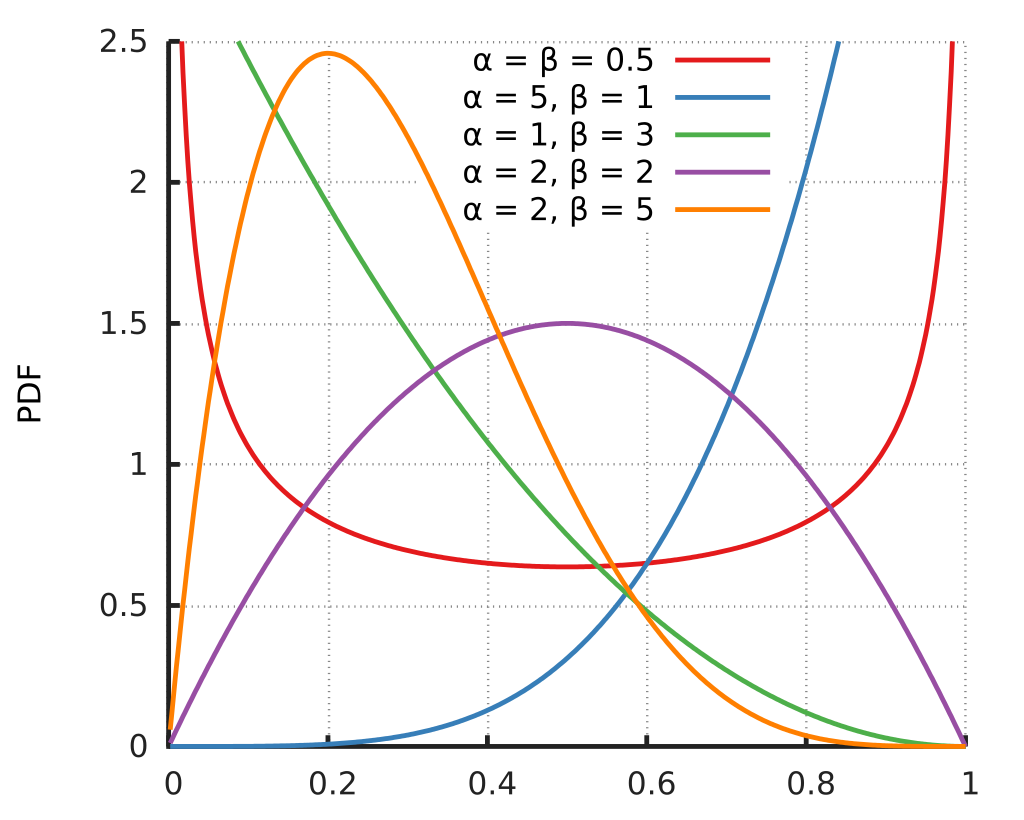
\includegraphics[scale=0.25]{img/beta-distribution.png}
    \caption{Gęstość rozkładu beta dla różnych parametrów}
\end{figure}

Na ćwiczeniach pokazywaliśmy fakt, który warto znać, a mianowicie
\[
    \expected{\Beta(\alpha, \beta)} = \frac{\alpha}{\alpha + \beta}
\]

Ponadto mamy jeszcze jedną własność, którą można zauważyć na rysunku
\begin{itemize}
    \item dla \( \alpha, \beta < 1 \) rozkład jest bimodalny 
    \item dla \( \alpha, \beta \geq 1 \) rozkład jest unimodalny
    \item dla \( \alpha = \beta \) rozkład jest symetryczny względem \( x = \frac{1}{2} \)
\end{itemize}

\subsection{Rozkłady sprzężone}
Aby nam się łatwiej liczyło wprowadzamy coś takiego jak \textbf{rozkład sprzężony}, czyli taki rozkład aprioryczny dla rozkładu próby, dla którego rozkład a posteriori i rozkład a priori jest taki sam.

\begin{center}
    \begin{tabular}{c c c}
         rozkład próby & a priori & a posteriori  \\
         \hline
         dwumianowy & beta & beta \\
         Poissona & gamma & gamma \\
         geometryczny & beta & beta \\
         wielomianowy & Dirichleta & Dirichleta \\
         wykładniczy & gamma & gamma \\
         normalny & normalny & normalny \\
    \end{tabular}
\end{center}

Jest to głównie potrzebne po to aby nam się prościej liczyło.

\subsection{Estymator}

\begin{definition}
\textbf{Estymator} to dowolna wartość szacowanego parametru obliczona na podstawie jakiejś próbki. Dla parametru \( \theta \) będziemy oznaczać estymator przez \( \widehat \theta \)
\end{definition}

\begin{definition}
\textbf{Obciążenie estymatora} \( \widehat \theta \) parametru \( \theta \) definiujemy jako
\[
    \bias(\widehat \theta) = \expected{\widehat \theta} - \theta
\]

Mówimy, że estymator jest \textbf{obciążony} jeśli \( \bias(\theta) \neq 0 \)
\end{definition}

\subsection{Twierdzenie Bayesa}

Ustalmy dowolny model parametryczny.
Niech \( \theta \) będzie zmienną opisującą parametr modelu.
Niech \( D \) będzie zmienną losową, która opisuje obserwacje zwracane przez ten model.
Zachodzi wtedy wzór Bayesa na prawdopodobieństwo warunkowe:
\[
    \prob(\theta = t \given D = d) = \frac{P(D = d \given \theta = t) \cdot P(\theta =t )}{P(D = d)}
\]

Dzięki temu jesteśmy w stanie na podstawie obserwacji szacować parametr naszego modelu.

Podobnie jeśli \( \theta \) i \( D \) są zmiennymi ciągłymi to
\[
    f_{\theta \given D = d} = \frac{f_{D \given \theta = t}(d) \cdot f_\theta(t)}{f_D(d)}
\]

Nadużywając notacji będziemy zapisywać obie te sytuacje jednocześnie, przyjmując przy tym że \( p(X) \) jest rozkładem zmiennej \( X \)

\[
    p(\theta \given D) = \frac{p(D \given \theta) \cdot p(\theta)}{p(D)}
\]

Nazywamy elementy tego wzoru:
\begin{itemize}
    \item \( p(\theta) \) to \textbf{prawdopodobieństwo a priori}, czyli co wiemy (zakładamy) o \( \theta \) jeśli nie mamy żadnych obserwacji
    \item \( p(D \mid \theta) \) to \textbf{wiarygodność}, czyli jak dobrze model z parametrem \( \theta \) przewiduje dane z obserwacji
    \item \( p(\theta \mid D) \) to \textbf{prawdopodobieństwo a posteriori}, czyli co powinniśmy zakładać o \( \theta \) jeśli poczyniliśmy już obserwacje
    \item \( p(D) \) to \textbf{wiarygodność brzegowa}, czyli jakie w ogólności jest prawdopodobieństwo uzyskania naszych obserwacji
    
    \[
        p(D) = \int_{\im \theta} p(D \mid \theta)p(\theta)d\theta 
    \]
\end{itemize}

Warto tutaj zauważyć, że \( p(D) \) jest niezależne od \( \theta \) tj. zależy jedynie od samego modelu, a nie od konkretnego parametru.
